\documentclass[12pt]{article}
\usepackage{geometry}                % See geometry.pdf to learn the layout options. There are lots.
\geometry{letterpaper}                   % ... or a4paper or a5paper or ... 
%\geometry{landscape}                % Activate for for rotated page geometry
\usepackage[parfill]{parskip}    % Activate to begin paragraphs with an empty line rather than an indent
\usepackage{daves,fancyhdr,natbib,graphicx,dcolumn,amsmath,lastpage,url}
\usepackage{amsmath,amssymb,epstopdf,longtable}
\usepackage{paralist}  % need to properly formulate standard answer blocks
\usepackage[final]{pdfpages}
\DeclareGraphicsRule{.tif}{png}{.png}{`convert #1 `dirname #1`/`basename #1 .tif`.png}
\pagestyle{fancy}
\lhead{CE 3305 Fluid Mechanics; Exercise Set 2}
\rhead{Name:\_\_\_\_\_\_\_\_\_\_\_\_\_\_\_\_\_\_\_\_\_\_\_\_\_\_\_\_\_\_\_\_\_\_}
\lfoot{REVISION A}
\cfoot{}
\rfoot{Page \thepage\ of \pageref{LastPage}}
\renewcommand\headrulewidth{0pt}
%%%%%%%%%%%%%%%%%%%%%%%%%%%%%%%%%%%%
\begin{document}
%%%%%%%%%%%%%%%%%%%%%%%%%%%%%%%%%%%
\begingroup
\begin{center}
{\textbf{{ CE 3305 Engineering Fluid Mechanics} \\ Exercise Set 2 \\ Summer 2018 -- GERMANY} }
\end{center}
\endgroup
\begingroup
~\newline
\textbf{Purpose} : Use compressibility to relate pressure change to volume change.  Apply definition of viscosity in Newtonian fluid. \\
\textbf{Assessment Criteria} : Completion, plausible solutions, use \textbf{R} as a calculator. \\~\\
\textbf{Exercises}

\begin{enumerate}
\item (Problem 2.13 pg 55)
Calculate the pressure increase ($\Delta p$) required to reduce the volume of a mass of water by 2-percent (2 $\%$) 

\item (Problem 2.35 pg 56)
Figure \ref{fig:SlidingPlateViscosity} is a schematic of a sliding plate viscometer used to measure the viscosity of a fluid. 
The top plate is moving to the right with a constant velocity of 10 meters per second in response to a force of 3 Newtons.
What is the viscosity of the fluid?\footnote{Assume a linear velocity distribution.}
\begin{figure}[htbp] %  figure placement: here, top, bottom, or page
   \centering
   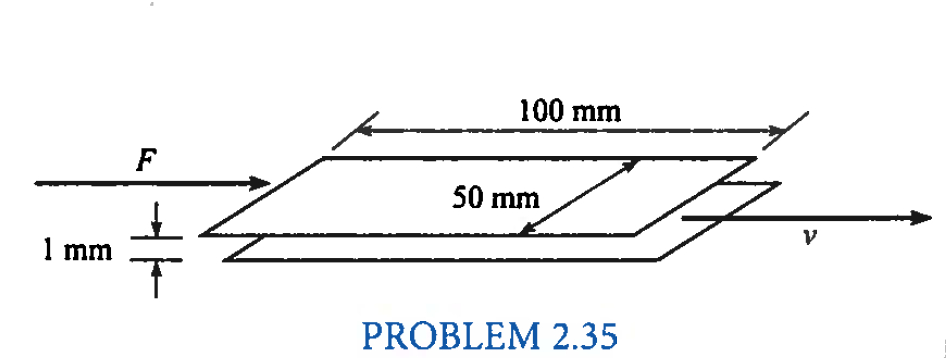
\includegraphics[width=4in]{SlidingPlateViscosity.jpg} 
   \caption{Sliding Plate Viscometer}
   \label{fig:SlidingPlateViscosity}
\end{figure}

\end{enumerate}


\end{document}  